\section{Topics covered}
\begin{itemize}
\item The process improvement process
\item Process measurement
\item Process analysis
\item Process change
\item The CMMI process improvement framework
\end{itemize}



\section{Process improvement}
\begin{itemize}
\item Many software companies have turned to software process improvement as a way of enhancing the quality of their software, reducing costs or accelerating their development processes.
\item Process improvement means understanding existing processes and changing these processes to increase product quality and/or reduce costs and development time.
\end{itemize}



\section{Approaches to improvement}
\begin{itemize}
\item The process maturity approach, which focuses on improving process and project management and introducing good software engineering practice.

   \item The level of process maturity reflects the extent to which good technical and management practice has been adopted in organizational software development processes.

\item The agile approach, which focuses on iterative development and the reduction of overheads in the software process.

   \item The primary characteristics of agile methods are rapid delivery of functionality and responsiveness to changing customer requirements.
\end{itemize} \section{Process and product quality}
\begin{itemize}

\item Process quality and product quality are closely
related and process improvement benefits arise because the quality of the product depends on its development process.

\item A good process is usually required to produce a good product.

\item For manufactured goods, process is the principal quality determinant.

\item For design-based activities, other factors are also involved, especially the capabilities of the designers.
\end{itemize}

\section{Factors affecting software product quality}
\begin{figure}[h!]
    \centering
    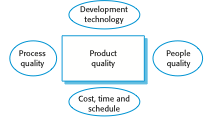
\includegraphics[width = 0.8\textwidth]{./figures/L9_1.png}
    \caption{}
    \label{fig:L9_1}
\end{figure}


\section{Quality factors}
\begin{itemize}



\item For large projects with ‘average’ capabilities, the development process determines product quality.

\item For small projects, the capabilities of the developers is the main determinant.

\item The development technology is particularly significant for small projects.

\item In all cases, if an unrealistic schedule is imposed then product quality will suffer.


\end{itemize}

\section{Process improvement process}
\begin{itemize}

\item There is no such thing as an ‘ideal’ or ‘standard’ software process that is applicable in all organizations or for all software products of a particular type.

   \item You will rarely be successful in introducing process improvements if you simply attempt to change the process to one that is used elsewhere.
   \item You must always consider the local environment and culture and how this may be affected by process change proposals.

\item Each company has to develop its own process depending on its size, the background and skills of its staff, the type of software being developed, customer and market requirements, and the company culture.

\end{itemize}

\section{Improvement attributes}
\begin{itemize}

\item You also have to consider what aspects of the process that you want to improve.

\item Your goal might be to improve software quality and so you may wish to introduce new process activities that change the way software is developed and tested.

\item You may be interested in improving some attribute of the process itself (such as development time) and you have to decide which process attributes are the most important to your company.
\end{itemize}

\section{Process improvement stages}
\begin{itemize}


\item Process measurement

   \item Attributes of the current process are measured. These are a baseline for assessing improvements.

\item Process analysis

   \item The current process is assessed and bottlenecks and weaknesses are identified.

\item Process change

   \item Changes to the process that have been identified during the analysis are introduced.


\end{itemize}

\section{Process attributes}
\begin{table}[h!]
\centering
\begin{tabular}{ |p{3cm}|p{8cm}|  }
\hline
Process characteristic & Key issues \\
\hline
\hline
Understandability & To what extent is the process explicitly defined and how easy is it to understand the process definition?\\
\hline
Standardization & To what extent is the process based on a standard generic process? This may be important for some customers who require conformance with a set of defined process standards. To what extent is the same process used in all parts of a company?\\
\hline
Visibility & Do the process activities culminate in clear results, so that the progress of the process is externally visible?\\
\hline
Measurability & Does the process include data collection or other activities that allow process or product characteristics to be measured?\\
\hline
Supportability & To what extent can software tools be used to support the process activities?\\
\hline
Acceptability & Is the defined process acceptable to and usable by the engineers responsible for producing the software product?\\
\hline
Reliability & Is the process designed in such a way that process errors are avoided or trapped before they result in product errors?\\
\hline
Robustness & Can the process continue in spite of unexpected problems?\\
\hline
Maintainability & Can the process evolve to reflect changing organizational requirements or identified process improvements?\\
\hline
Rapidity & How fast can the process of delivering a system from a given specification be completed?\\
\hline
\end{tabular}

\label{table:T6_2}
\end{table}


\section{The process improvement cycle}
\begin{figure}[h!]
    \centering
    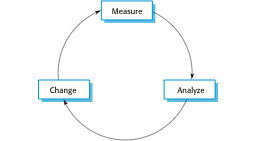
\includegraphics[width = 0.8\textwidth]{./figures/L9_2.png}
    \caption{}
    \label{fig:L9_2}
\end{figure}

\section{Process measurement}
\begin{itemize}

\item Wherever possible, quantitative process data should be collected

   \item However, where organisations do not have clearly defined process standards this is very difficult as you don’t know what to measure. A process may have to be defined before any measurement is possible.

\item Process measurements should be used to assess process improvements

   \item But this does not mean that measurements should drive the improvements. The improvement driver should be the organizational objectives.


\end{itemize}

\section{Process metrics}
\begin{itemize}




\item Time taken for process activities to be completed

   \item E.g. Calendar time or effort to complete an activity or process. \item Resources required for processes or activities
   \item E.g. Total effort in person-days.

\item Number of occurrences of a particular event    \item E.g. Number of defects discovered.

\end{itemize}

\section{Goal-Question-Metric Paradigm}
\begin{itemize}

\item Goals

   \item What is the organisation trying to achieve? The objective of process improvement is to satisfy these goals.

\item Questions

   \item Questions about areas of uncertainty related to the goals. You need process knowledge to derive these.

\item Metrics

   \item Measurements to be collected to answer the questions.



\end{itemize}

\section{GQM questions}
\begin{itemize}

\item The GQM paradigm is used in process improvement to help answer three critical questions:

   \item Why are we introducing process improvement?

   \item What information do we need to help identify and assess improvements?
   \item What process and product measurements are required to provide this information?



\end{itemize}

\section{The GQM paradigm}
\begin{figure}[h!]
    \centering
    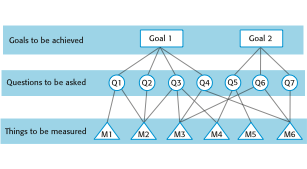
\includegraphics[width = 0.8\textwidth]{./figures/L9_3.png}
    \caption{}
    \label{fig:L9_3}
\end{figure}


\section{Process analysis}
\begin{itemize}

\item The study of existing processes to understand the relationships between parts of the process and to compare them with other processes.

\item Process analysis and process measurement are intertwined.

\item You need to carry out some analysis to know what to measure, and, when making measurements, you inevitably develop a deeper understanding of the process being measured.

\end{itemize}

\section{Process analysis objectives}
\begin{itemize}

\item To understand the activities involved in the process and the relationships between these activities.

\item To understand the relationships between the process activities and the measurements that have been made.

\item To relate the specific process or processes that you are analyzing to comparable processes elsewhere in the organization, or to idealized processes of the same type.


\end{itemize}

\section{Process analysis techniques}
\begin{itemize}
\item Published process models and process standards

   \item It is always best to start process analysis with an existing model. People then may extend and change this.

\item Questionnaires and interviews

   \item Must be carefully designed. Participants may tell you what they think you want to hear.

\item Ethnographic analysis

   \item Involves assimilating process knowledge by observation. Best for in-depth analysis of process fragments rather than for whole-process understanding.

\end{itemize}
\newpage
\section{Aspects of process analysis}
\begin{longtable}{ |p{2cm}|p{10cm}|  }
% \centering
% \begin{tabular}{ |p{2cm}|p{10cm}|  }
\hline
Process aspect & Questions \\
\hline
\hline
Adoption and standardization & Is the process documented and standardized across the organization? If not, does this mean that any measurements made are specific only to a single process instance? If processes are not standardized, then changes to one process may not be transferable to comparable processes elsewhere in the company.\\
\hline
Software engineering practice & Are there known, good software engineering practices that are not included in the process? Why are they not included? Does the lack of these practices affect product characteristics, such as the number of defects in a delivered software system?\\
\hline
Organizational constraints & What are the organizational constraints that affect the process design and the ways that the process is performed? For example, if the process involves dealing with classified material, there may be activities in the process to check that classified information is not included in any material due to be released to external organizations. Organizational constraints may mean that possible process changes cannot be made.\\
\hline
Communications & How are communications managed in the process? How do communication issues relate to the process measurements that have been made? Communication problems are a major issue in many processes and communication bottlenecks are often the reasons for project delays.\\
\hline
Introspection & Is the process reflective (i.e., do the actors involved in the process explicitly think about and discuss the process and how it might be improved)? Are there mechanisms through which process actors can propose process improvements?\\
\hline
Learning & How do people joining a development team learn about the software processes used? Does the company have process manuals and process training programs?\\
\hline
Tool support & What aspects of the process are and aren’t supported by software tools? For unsupported areas, are there tools that could be deployed cost-effectively to provide support? For supported areas, are the tools effective and efficient? Are better tools available?\\
\hline
% \end{tabular}
\caption{}
\label{table:T9_2}
\end{longtable}

\section{Process models}
\begin{itemize}
\item Process models are a good way of focusing attention on the activities in a process and the information transfer between these activities.

\item Process models do not have to be formal or complete – their purpose is to provoke discussion rather than document the process in detail.

\item Model-oriented questions can be used to help understand the process e.g.

   \item What activities take place in practice but are not shown in the model?
   \item Are there process activities, shown in the model, that you (the process actor) think are inefficient?

\end{itemize}

\section{Process exceptions}
\begin{itemize}


\item Software processes are complex and process models cannot effectively represent how to handle exceptions:

   \item Several key people becoming ill just before a critical review;
   \item A breach of security that means all external communications are out of action for several days;
   \item Organisational reorganisation;
   \item A need to respond to an unanticipated request for new proposals.

\item Under these circumstances, the model is suspended and managers use their initiative to deal with the exception.
\end{itemize}

\section{Key points}
\begin{itemize}


\item The goals of process improvement are higher product quality, reduced process costs and faster delivery of software.

\item The principal approaches to process improvement are agile approaches, geared to reducing process overheads, and maturity-based approaches based on better process management and the use of good software engineering practice.

\item The process improvement cycle involves process measurement, process analysis and modeling, and process change.

\item Measurement should be used to answer specific questions about the software process used. These questions should be based on organizational improvement goals.

\end{itemize}

\section{Process change}
\begin{itemize}

\item Involves making modifications to existing processes. \item This may involve:
   \item Introducing new practices, methods or processes;    \item Changing the ordering of process activities;    \item Introducing or removing deliverables;    \item Introducing new roles or responsibilities.
\item Change should be driven by measurable goals.
\section{The process change process}
\begin{figure}[h!]
    \centering
    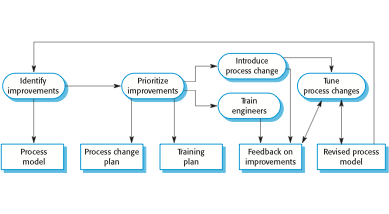
\includegraphics[width = 0.8\textwidth]{./figures/L9_4.png}
    \caption{}
    \label{fig:L9_4}
\end{figure}


\end{itemize}

\section{Process change stages}
\begin{itemize}

\item Improvement identification

   \item This stage is concerned with using the results of the process analysis to identify ways to tackle quality problems, schedule bottlenecks or cost inefficiencies that have been identified during process analysis.

\item Improvement prioritization

   \item When many possible changes have been identified, it is usually impossible to introduce them all at once, and you must decide which are the most important.

\item Process change introduction

   \item Process change introduction means putting new procedures, methods and tools into place and integrating them with other process activities.
\end{itemize}

\section{Process change stages}
\begin{itemize}

\item Process change training

   \item Without training, it is not possible to gain the full benefits of process changes. The engineers involved need to understand the changes that have been proposed and how to perform the new and changed processes.

\item Change tuning

   \item Proposed process changes will never be completely effective as soon as they are introduced. You need a tuning phase where minor problems can be discovered, and modifications to the process can be proposed and introduced.


\end{itemize}

\section{Process change problems}
\begin{itemize}

\item Resistance to change

   \item Team members or project managers may resist the introduction of process changes and propose reasons why changes will not work, or delay the introduction of changes. They may, in some cases, deliberately obstruct process changes and interpret data to show the ineffectiveness of proposed process change.

\item Change persistence

   \item While it may be possible to introduce process changes initially, it is common for process innovations to be discarded after a short time and for the processes to revert to their previous state.

\end{itemize}

\section{Resistance to change}
\begin{itemize}

\item Project managers often resist process change because any innovation has unknown risks associated with it.

   \item Project managers are judged according to whether or not their project produces software on time and to budget. They may prefer an inefficient but predictable process to an improved process that has organizational benefits, but which has short-term risks associated with it.

\item Engineers may resist the introduction of new processes for similar reasons, or because they see these processes as threatening their professionalism.

   \item That is, they may feel that the new pre-defined process gives them less discretion and does not recognize the value of their skills and experience.

\end{itemize}

\section{Change persistence}
\begin{itemize}

\item The problem of changes being introduced then subsequently discarded is a common one.

   \item Changes may be proposed by an ‘evangelist’ who believes strongly that the changes will lead to improvement. He or she may work hard to ensure the changes are effective and the new process is accepted.
   \item If the ‘evangelist’ leaves, then the people involved may therefore simply revert to the previous ways of doing things.

\item Change institutionalization is important

   \item This means that process change is not dependent on individuals but that the changes become part of standard practice in the company, with company-wide support and training.


\end{itemize}

\section{The CMMI process improvement framework}
\begin{itemize}
\item The CMMI framework is the current stage of work on process assessment and improvement that started at the Software Engineering Institute in the 1980s.

\item The SEI’s mission is to promote software technology transfer particularly to US defence contractors.

\item It has had a profound influence on process improvement    \item Capability Maturity Model introduced in the early 1990s.    \item Revised maturity framework (CMMI) introduced in 2001.



\end{itemize}

\section{The SEI capability maturity model}
\begin{itemize}

\item Initial

   \item Essentially uncontrolled \item Repeatable
   \item Product management procedures defined and used \item Defined
   \item Process management procedures and strategies defined and used

\item Managed

   \item Quality management strategies defined and used \item Optimising
   \item Process improvement strategies defined and used

\end{itemize}

\section{Process capability assessment}
\begin{itemize}

\item Intended as a means to assess the extent to which an organisation’s processes follow best practice.

\item By providing a means for assessment, it is possible to identify areas of weakness for process improvement.

\item There have been various process assessment and improvement models but the SEI work has been most influential.

\end{itemize}

\section{The CMMI model}
\begin{itemize}

\item An integrated capability model that includes software and systems engineering capability assessment.

\item The model has two instantiations

   \item Staged where the model is expressed in terms of capability levels;
   \item Continuous where a capability rating is computed.


\end{itemize}

\section{CMMI model components}
\begin{itemize}

\item Process areas

   \item 24 process areas that are relevant to process capability and improvement are identified. These are organised into 4 groups.

\item Goals

   \item Goals are descriptions of desirable organisational states. Each process area has associated goals.

\item Practices

   \item Practices are ways of achieving a goal - however, they are advisory and other approaches to achieve the goal may be used.


\end{itemize}
\newpage
\section{Process areas in the CMMI}
\begin{longtable}{ |p{3cm}|p{8cm}|  }
% \centering
% \begin{tabular}{ |p{3cm}|p{8cm}|  }
\hline
Category & Process area \\
\hline
\hline
Process management &
\begin{itemize}
\item Organizational process definition (OPD)
\item Organizational process focus (OPF)
\item Organizational training (OT)
\item Organizational process performance (OPP)
\item Organizational innovation and deployment (OID)
\end{itemize}\\
\hline
Project management &
\begin{itemize}
  \item Project planning (PP)
  \item Project monitoring and control (PMC)
  \item Supplier agreement management (SAM)
  \item Integrated project management (IPM)
  \item Risk management (RSKM)
  \item Quantitative project management (QPM)
\end{itemize}\\
\hline
Engineering &
\begin{itemize}
  \item Requirements management (REQM)
  \item Requirements development (RD)
  \item Technical solution (TS)
  \item Product integration (PI)
  \item Verification (VER)
  \item Validation (VAL)
\end{itemize}\\
\hline
Support &
\begin{itemize}
  \item Configuration management (CM)
  \item Process and product quality management (PPQA)
  \item Measurement and analysis (MA)
  \item Decision analysis and resolution (DAR)
  \item Causal analysis and resolution (CAR)
\end{itemize}\\
\hline
% \end{tabular}
\caption{}
\label{table:T9_3}
\end{longtable}

\section{Goals and associated practices in the CMMI}
\begin{longtable}{ |p{3cm}|p{8cm}|  }
% \centering
% \begin{tabular}{ |p{3cm}|p{8cm}|  }
\hline
Category & Process area \\
\hline
\hline
Process management &
\begin{itemize}
\item Organizational process definition (OPD)
\item Organizational process focus (OPF)
\item Organizational training (OT)
\item Organizational process performance (OPP)
\item Organizational innovation and deployment (OID)
\end{itemize}\\
\hline
Project management &
\begin{itemize}
  \item Project planning (PP)
  \item Project monitoring and control (PMC)
  \item Supplier agreement management (SAM)
  \item Integrated project management (IPM)
  \item Risk management (RSKM)
  \item Quantitative project management (QPM)
\end{itemize}\\
\hline
Engineering &
\begin{itemize}
  \item Requirements management (REQM)
  \item Requirements development (RD)
  \item Technical solution (TS)
  \item Product integration (PI)
  \item Verification (VER)
  \item Validation (VAL)
\end{itemize}\\
\hline
Support &
\begin{itemize}
  \item Configuration management (CM)
  \item Process and product quality management (PPQA)
  \item Measurement and analysis (MA)
  \item Decision analysis and resolution (DAR)
  \item Causal analysis and resolution (CAR)
\end{itemize}\\
\hline
% \end{tabular}
\caption{}
\label{table:T9_3}
\end{longtable}
\newpage
\section{Goals and associated practices in the CMMI}

\begin{table}[h!]
\centering
\begin{tabular}{ |p{5cm}|p{5cm}|  }
\hline
Goal & Associated practices \\
\hline
The requirements are analyzed and validated, and a definition of the required functionality is developed. & Analyze derived requirements systematically to ensure that they are necessary and sufficient.\\
\hline
& Validate requirements to ensure that the resulting product will perform as intended in the user’s environment, using multiple techniques as appropriate.\\
\hline
Root causes of defects and other problems are systematically determined. & Select the critical defects and other problems for analysis.\\
\hline
 & Perform causal analysis of selected defects and other problems and propose actions to address them.\\
 \hline
The process is institutionalized as a defined process. & Establish and maintain an organizational policy for planning and performing the requirements development process.\\
\hline
\end{tabular}

\label{table:T9_4}
\end{table}

\section{CMMI assessment}
\begin{itemize}

\item Examines the processes used in an organisation and assesses their maturity in each process area.

\item Based on a 6-point scale:    \item Not performed;    \item Performed;
   \item Managed;    \item Defined;
   \item Quantitatively managed;    \item Optimizing.

\end{itemize}

\section{Examples of goals in the CMMI}

\begin{table}[h!]
\centering
\begin{tabular}{ |p{5cm}|p{5cm}|  }
\hline
Goal & Process area \\
\hline
\hline
Corrective actions are managed to closure when the project’s performance or results deviate significantly from the plan. & Project monitoring and control (specific goal)\\
\hline
Actual performance and progress of the project are monitored against the project plan. & Project monitoring and control (specific goal)\\
\hline
The	requirements	are	analyzed	and validated, and a definition of the required functionality is developed. & Requirements development (specific goal)\\
\hline
Root causes of defects and other problems are systematically determined. & Causal analysis and resolution (specific goal)\\
\hline
The process is institutionalized as a defined process. & Generic goal\\
\hline
\end{tabular}

\label{table:T9_5}
\end{table}





\section{The staged CMMI model}
\begin{itemize}


\item Comparable with the software CMM.

\item Each maturity level has process areas and goals. For example, the process area associated with the managed level include:

   \item Requirements management;    \item Project planning;
   \item Project monitoring and control;    \item Supplier agreement management;    \item Measurement and analysis;
   \item Process and product quality assurance.

\end{itemize}
\newpage
\section{The CMMI staged maturity model}
\begin{figure}[h!]
    \centering
    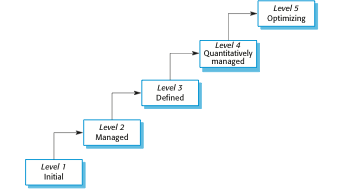
\includegraphics[width = 0.8\textwidth]{./figures/L9_5.png}
    \caption{}
    \label{fig:L9_5}
\end{figure}

\section{Institutional practices}
\begin{itemize}




\item Institutions operating at the managed level should have institutionalised practices that are geared to standardisation.

   \item Establish and maintain policy for performing the project management process;
   \item Provide adequate resources for performing the project management process;
   \item Monitor and control the project planning process;
   \item Review the activities, status and results of the project planning process.

\end{itemize}

\section{The continuous CMMI model}
\begin{itemize}
\item This is a finer-grain model that considers individual or groups of practices and assesses their use.

\item The maturity assessment is not a single value but is a set of values showing the organisations maturity in each area.

\item The CMMI rates each process area from levels 1 to 5.

\item The advantage of a continuous approach is that organisations can pick and choose process areas to improve according to their local needs.

\end{itemize}

\section{A process capability profile}
\begin{figure}[h!]
    \centering
    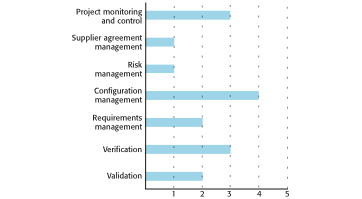
\includegraphics[width = 0.8\textwidth]{./figures/L9_6.png}
    \caption{}
    \label{fig:L9_6}
\end{figure}

\section{Key points}
\begin{itemize}

\item The CMMI process maturity model is an integrated process improvement model that supports both staged and continuous process improvement.

\item Process improvement in the CMMI model is based on reaching a set of goals related to good software engineering practice and describing, standardizing and controlling the practices used to achieve these goals.

\item The CMMI model includes recommended practices that may be used, but these are not obligatory.
\end{itemize}
